% ===================================================================
%  بخش ۴ — نتایج تست دوم و بحث
% ===================================================================
\section{نتایج و بحث}
\label{sec:results}

\subsection{پاسخ دوقطبی طولی و فاکتور پورسل}
\label{sec:results-purcell}

در حالت اصلی A، دوقطبی طولی در فاصله پنج نانومتری از نوک نانومیله با مد
پلاسمونی طولی جفت شد. نمودار خروجی تست دوم، قله فاکتور پورسل را در حدود
$\lambda\simeq\nm{610}$ و با مقدار تقریبی $\Fp\simeq1490$ نشان می‌دهد.
این مقدار افزایش بیش از سه مرتبه بزرگی نرخ واپاشی کل را نشان می‌دهد.
مکان قله در ناحیه تشدید طولی نانومیله قرار دارد، در حالی که ارتفاع آن به
مش، نمونه‌برداری منبع و نرمال‌سازی عددی حساس‌تر است.

شکل~\ref{fig:purcell} طیف کامل نمایش‌داده‌شده در خروجی Lumerical حالت A را
نشان می‌دهد. چون جدول متنی این حالت در دسترس نبود، منحنی برای صفحه‌آرایی
مقاله از روی تصویر خروجی رقم‌زنی و بازترسیم شد؛ بنابراین شکل طیفی معتبر
است، ولی مقادیر میان‌نقطه‌ای آن نباید با دقت فایل خام تفسیر شوند. کنترل
فضای آزاد در $\nm{610}$ مقدار $F_{p,B}=0.9686$ می‌دهد؛ اگر صرفاً این خطای
پایه اصلاح شود، قله A حدود $1538$ برآورد می‌شود. عدد اصلی مقاله همان
خروجی خام $\Fp\simeq1490$ است و مقدار تصحیح‌شده فقط برآورد خطای عددی است.

\begin{figure}[htbp]
 \centering
 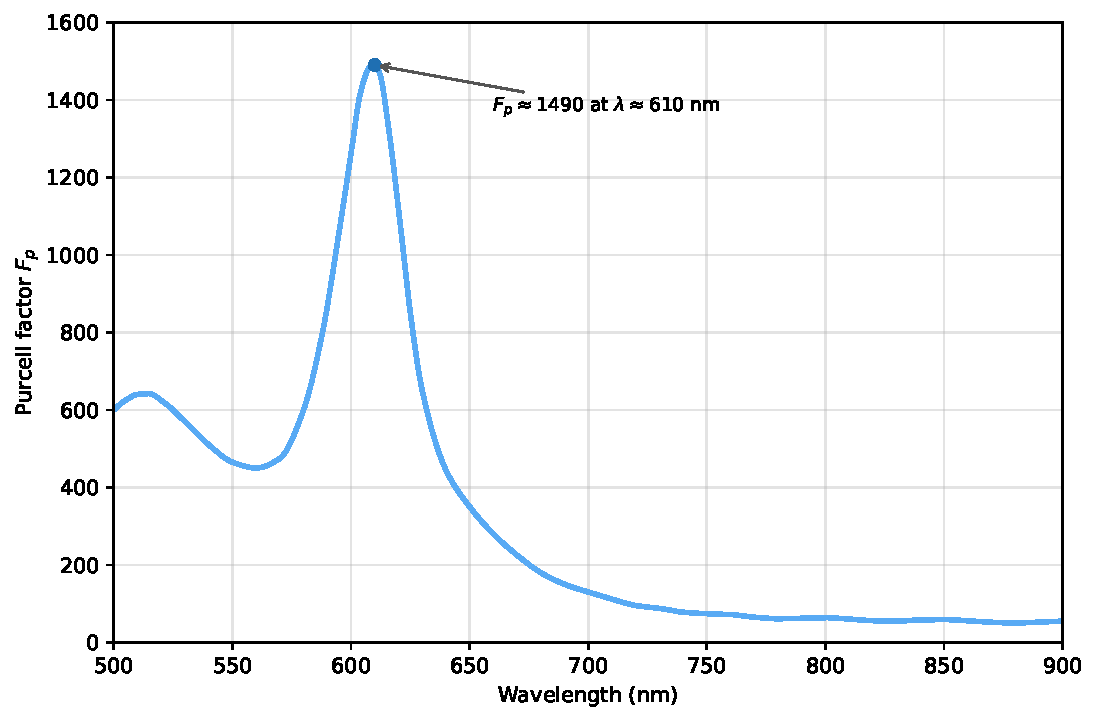
\includegraphics[width=0.88\linewidth]{figures/Test2_A_Purcell_full.pdf}
 \caption{طیف فاکتور پورسل حالت اصلی A برای نانومیله و دوقطبی طولی،
 رقم‌زنی و بازترسیم‌شده از تصویر خروجی Lumerical تست دوم. قله تقریبی
 $\Fp\simeq1490$ در حدود $\nm{610}$ قرار دارد.}
 \label{fig:purcell}
\end{figure}

\subsection{توان تابشی و موازنه انرژی}
\label{sec:results-radiated}

بیشینه تقویت توان تابشی حالت A برابر
$T_{\max}=119.219$ در حدود $\nm{616}$ به دست آمد
(شکل~\ref{fig:radiated}). قله تابشی تقریباً شش نانومتر سرخ‌تر از قله
پورسل است. این جدایی نشان می‌دهد که بیشینه کار انجام‌شده توسط چشمه و
بیشینه انرژی خارج‌شده از جعبه شار دقیقاً در یک طول‌موج رخ نمی‌دهند؛ جذب
اهمی طلا و وابستگی طیفی برون‌کوپل‌شدن میدان نزدیک در این تفاوت نقش دارند
\cite{bharadwaj2009optical}.

\begin{figure}[htbp]
 \centering
 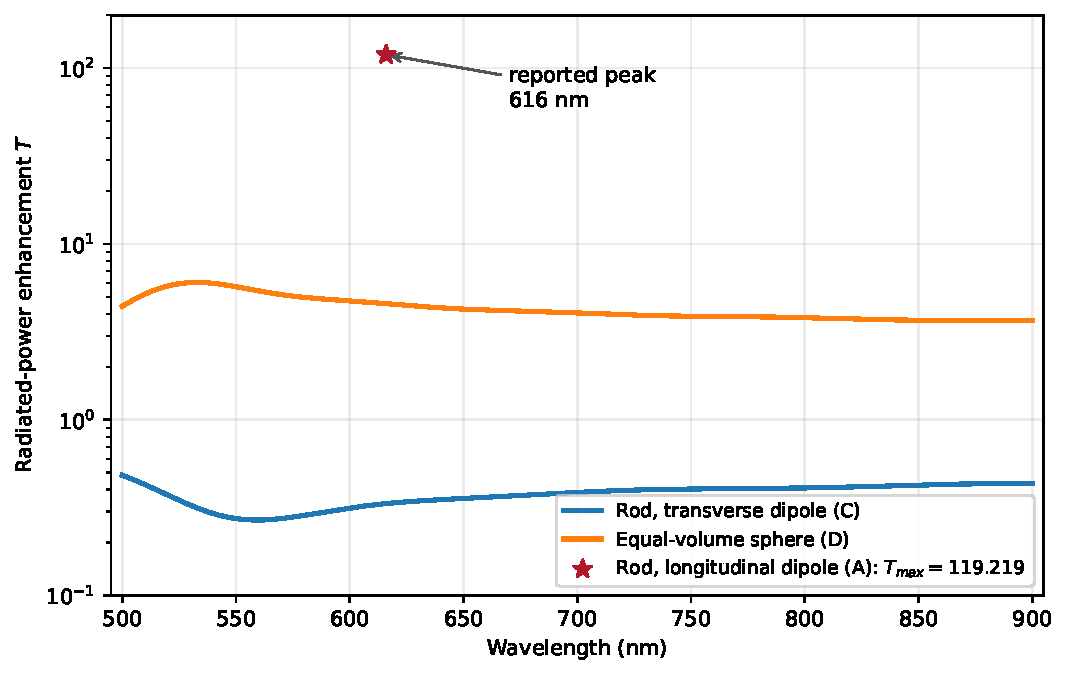
\includegraphics[width=0.88\linewidth]{figures/Test2_Radiated.pdf}
 \caption{تقویت توان تابشی تست دوم. ستاره قله گزارش‌شده حالت طولی A و
 منحنی‌ها خروجی کامل کنترل‌های C و D هستند. مقادیر هر سه حالت با تعریف
 خام $T=P_{\mathrm{rad}}/P_0$ رسم شده‌اند.}
 \label{fig:radiated}
\end{figure}

چون $\Fp$ و $T$ حالت A در دو طول‌موج متفاوت به بیشینه می‌رسند، تقسیم
مستقیم دو قله، راندمان طیفی دقیق نیست. بااین‌حال می‌توان یک کران معتبر
به دست آورد. در طول‌موج قله پورسل، توان تابشی نمی‌تواند از بیشینه کلی خود
بزرگ‌تر باشد؛ بنابراین
\begin{equation}
 \eta_a(\lambda_{F_p})=\frac{T(\lambda_{F_p})}{1490}
 \leq\frac{119.219}{1490}\simeq 8.0\%,
 \label{eq:eta-bound}
\end{equation}
و در نتیجه دست‌کم حدود ۹۲ درصد توان کل در آن طول‌موج وارد کانال‌های
غیرتابشی می‌شود. به‌طور مشابه،
\begin{equation}
 \frac{P_{\mathrm{loss}}(\lambda_{F_p})}{P_0}
 \geq1490-119.219=1370.781 .
 \label{eq:loss-bound}
\end{equation}
این بیان، برخلاف کم‌کردن دو قله در طول‌موج‌های متفاوت، یک کران فیزیکی
صحیح است و نتیجه اصلی یعنی غلبه خاموشی غیرتابشی در گپ پنج‌نانومتری را
حفظ می‌کند \cite{anger2006enhancement}.

\subsection{کنترل جهت‌گیری دوقطبی}
\label{sec:results-orientation}

حالت C اثر چرخاندن دوقطبی از راستای طولی به راستای عرضی را، بدون تغییر
هندسه و فاصله، اندازه می‌گیرد. قله خام آن
$F_p=239.235$ در $\nm{508}$ است، ولی توان تابشی در همان نقطه فقط
$T=0.4387$ و راندمان $0.183\%$ است. پس قله آبی C عمدتاً افزایش LDOS همراه
با جذب شدید است، نه یک تشدید تابشی کارآمد. پس از تصحیح با B، قله پورسل C
به $246.81$ در $\nm{506}$ می‌رسد.

در حوالی تشدید طولی، اختلاف بسیار بزرگ‌تر است. در $\nm{610}$ مقدار خام C
برابر $F_p=36.382$ است؛ بنابراین قله A تقریباً ۴۱ برابر بزرگ‌تر است. در
$\nm{616}$ نیز $T_C=0.3330$ است و بیشینه A حدود ۳۵۸ برابر آن است. این
کنترل مستقیم نشان می‌دهد پاسخ نانومیله یک کمیت همسانگرد نیست و جهت
دوقطبی باید صریحاً گزارش شود. بااین‌حال C کاملاً بدون جفت‌شدگی نیست؛ بیان
دقیق آن است که دوقطبی طولی با مد دوقطبی طولی نانومیله \emph{بسیار
مؤثرتر} از دوقطبی عرضی جفت می‌شود.

\subsection{کنترل کره هم‌حجم}
\label{sec:results-shape}

برای جداکردن اثر شکل از مقدار ماده، حالت D با کره‌ای به شعاع
$\nm{15.874}$ اجرا شد که حجمی برابر نانومیله دارد. قله خام کره
$F_p=658.738$ در $\nm{508}$ و قله تابشی آن $T=6.033$ در $\nm{532}$ است.
پس از تصحیح پایه، این دو قله به‌ترتیب $679.23$ و $6.063$ می‌شوند. در
$\nm{610}$ مقدار خام $F_p$ کره $96.131$ است؛ یعنی پاسخ طولی A تقریباً
۱۵٫۵ برابر بزرگ‌تر است. در $\nm{616}$ نیز $T_D=4.569$ و تقویت تابشی A
حدود ۲۶ برابر آن است. بنابراین تقویت نزدیک ۶۱۰ نانومتر صرفاً پیامد حجم
طلا نیست، بلکه به شکل کشیده و مد پلاسمونی طولی وابسته است. طیف کامل و
تصحیح‌شده کنترل‌های C و D در شکل~\ref{fig:cd-controls} آمده است.

\begin{figure}[htbp]
 \centering
 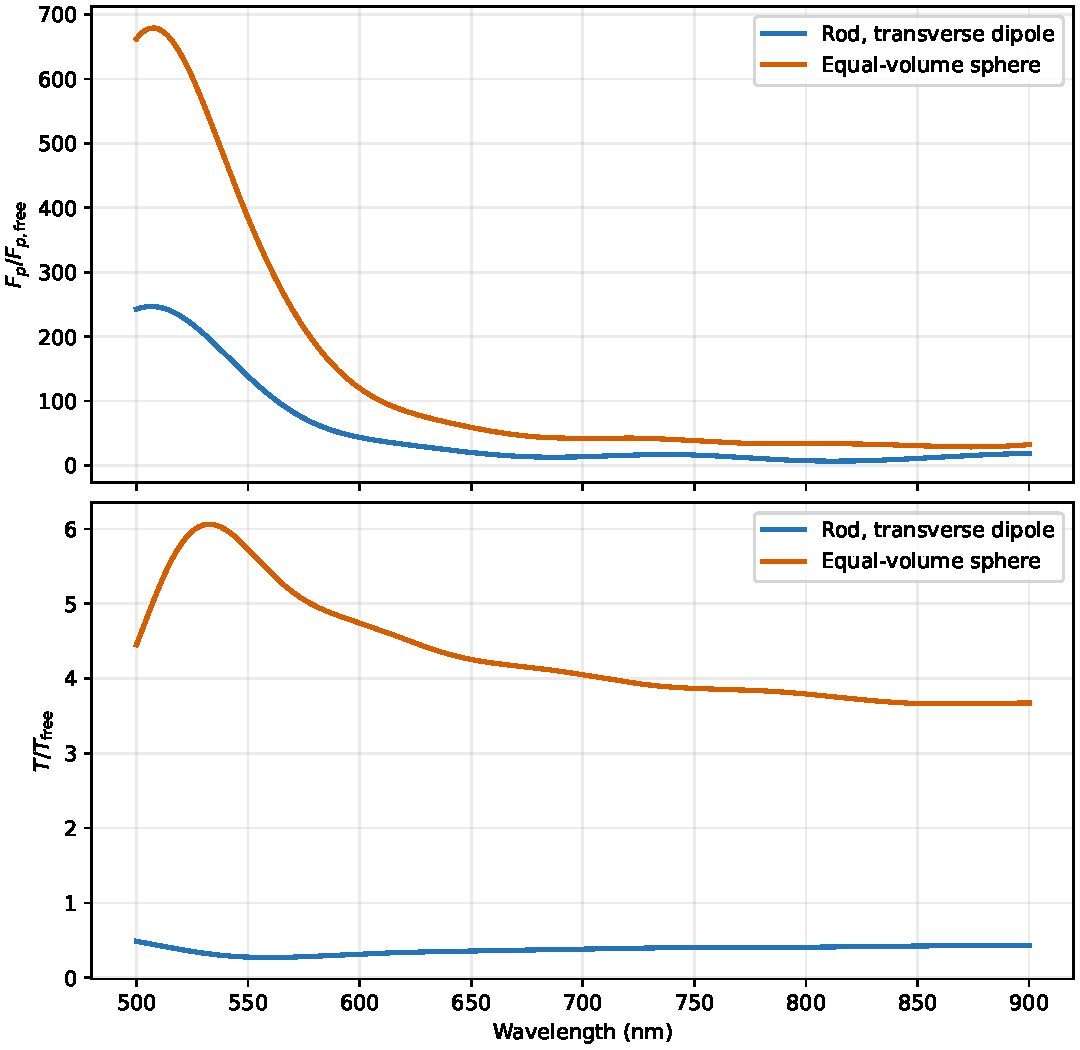
\includegraphics[width=0.92\linewidth]{figures/Test2_CD_Controls.pdf}
 \caption{طیف‌های تصحیح‌شده با مرجع فضای آزاد برای نانومیله با دوقطبی
 عرضی C و کره هم‌حجم D: فاکتور پورسل (بالا) و تقویت توان تابشی (پایین).
 این منحنی‌ها مستقیماً از فایل‌های ۲۰۱ نقطه‌ای Lumerical رسم شده‌اند.}
 \label{fig:cd-controls}
\end{figure}

\subsection{میدان نزدیک و محدودیت نمایش}
\label{sec:results-nearfield}

نقشه‌های میدان موجود C و D در شکل~\ref{fig:nearfield} با مقیاس لگاریتمی،
مرز هندسه و محل دوقطبی ترسیم شده‌اند. بیشینه C در
$(x,z)\simeq(0,\nm{35.08})$ و بیشینه D در
$(0,\nm{21.02})$ قرار دارد که با مکان چشمه‌ها سازگار است. میدان C در
$\nm{610}$ و میدان D در $\nm{530}$ ثبت شده‌اند؛ ازاین‌رو رنگ و مقدار
بیشینه دو پنل نباید به‌عنوان مقایسه مستقیم دامنه میدان تفسیر شود.

\begin{figure}[htbp]
 \centering
 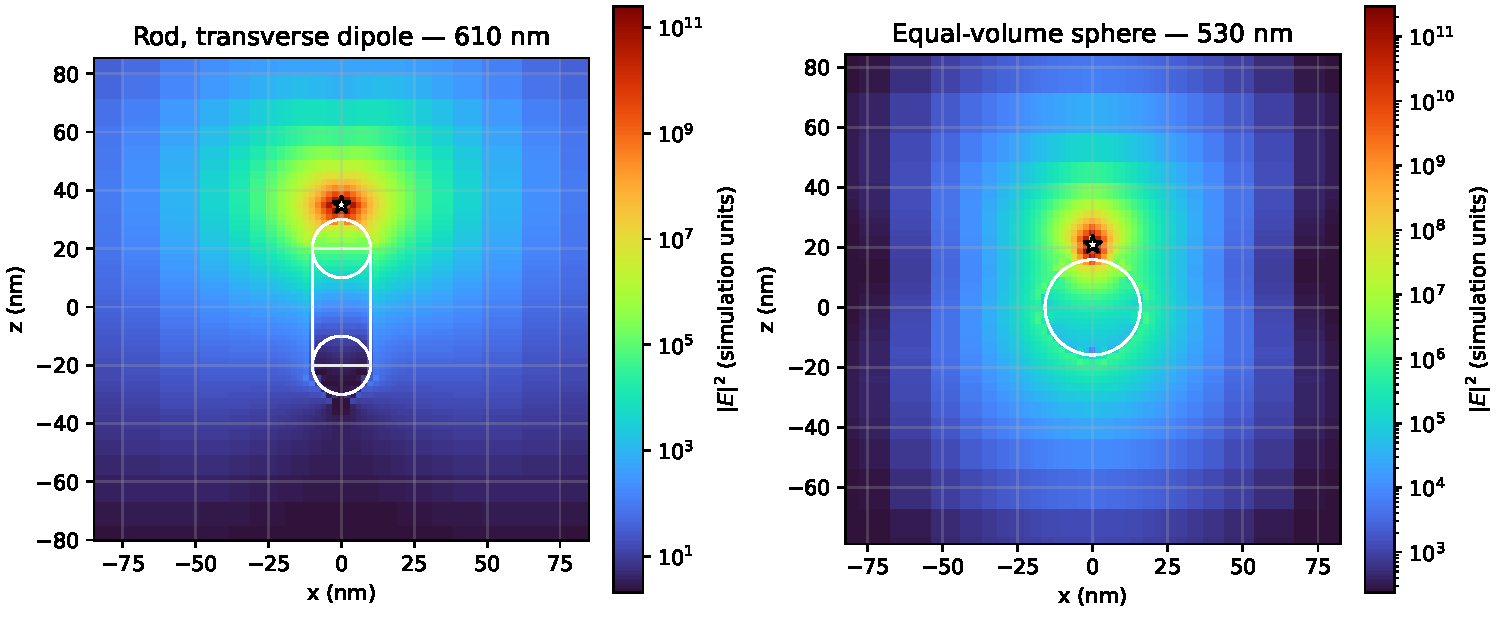
\includegraphics[width=0.98\linewidth]{figures/Test2_Nearfield_controls.pdf}
 \caption{نقشه لگاریتمی $|E|^2$ برای کنترل دوقطبی عرضی C در ۶۱۰ نانومتر
 (چپ) و کره هم‌حجم D در ۵۳۰ نانومتر (راست). خط سفید مرز فلز و ستاره محل
 دوقطبی است. طول‌موج و مقیاس رنگ دو پنل متفاوت‌اند.}
 \label{fig:nearfield}
\end{figure}

تمرکز بیشینه دقیقاً روی چشمه نقطه‌ای، بخشی از میدان نزدیک و تکین خود
دوقطبی است؛ بنابراین یک لکه روشن به‌تنهایی اثبات مود نیست. شناسایی مود
طولی در این پژوهش عمدتاً بر پاسخ طیفی A، اختلاف شدید A و C و مقایسه با
کره هم‌حجم تکیه دارد، نه فقط بر بیشینه یک پیکسل میدان.

\subsection{جمع‌بندی اعتبار عددی}
\label{sec:results-validity}

کنترل B برای T بسیار مطلوب است: $T_B$ در بازه ۵۰۰ تا ۹۰۰ نانومتر تقریباً
بین ۰٫۹۹۳ و ۱٫۰۰۳ باقی می‌ماند. در مقابل، $F_{p,B}$ مطابق
شکل~\ref{fig:free-baseline} تا ۱٫۱۳۳ تغییر می‌کند و وجود خطای پایه وابسته
به طول‌موج را نشان می‌دهد.

\begin{figure}[htbp]
 \centering
 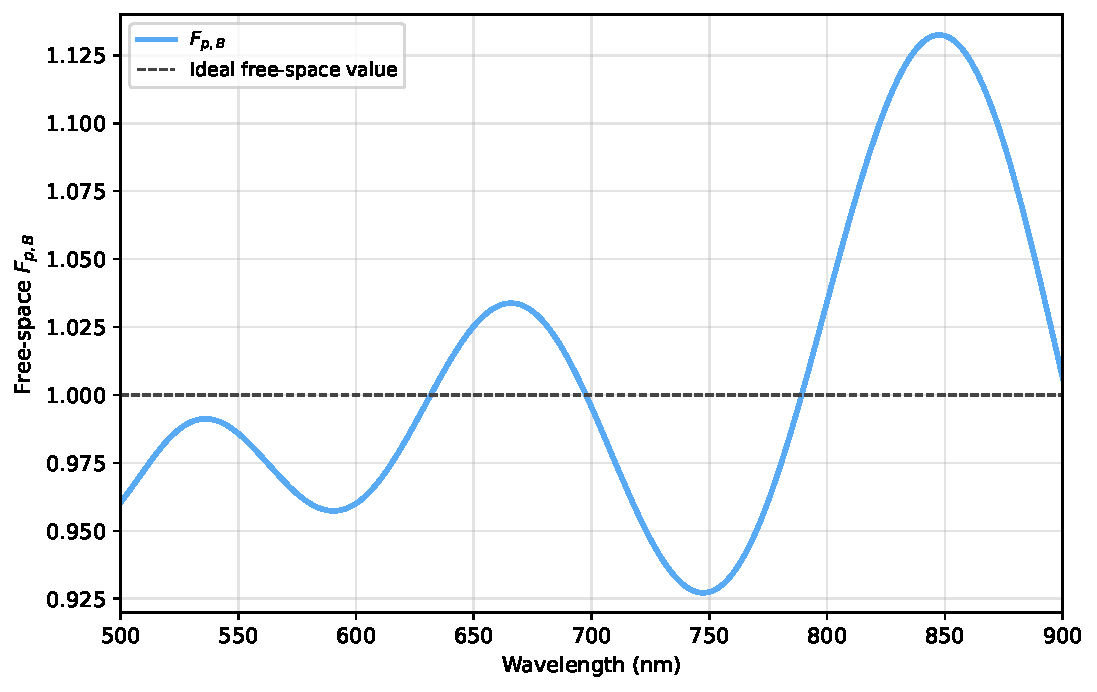
\includegraphics[width=0.84\linewidth]{figures/Test2_B_Freespace.pdf}
 \caption{خروجی فاکتور پورسل مرجع فضای آزاد B. خط‌چین مقدار ایده‌آل یک را
 نشان می‌دهد. انحراف طیفی از یک، عدم‌قطعیت عددی نرمال‌سازی را مشخص می‌کند.}
 \label{fig:free-baseline}
\end{figure}

این خطا نتیجه کیفی
مقایسه A، C و D را تغییر نمی‌دهد، ولی همراه با نبود آزمون همگرایی مش،
دقت اعداد قله را محدود می‌کند. ازاین‌رو اعداد تست دوم با تعداد رقم متناسب
گزارش شدند: مقدار پورسل A تقریبی، مقدار T مطابق خروجی موجود، و نتایج کامل
C و D با تصحیح طول‌موج‌به‌طول‌موج کنترل شدند. اجرای مش‌های ۳ و ۱٫۵
نانومتر و گپ‌های دیگر در اسکریپت تعریف شده، ولی در مجموعه حاضر اجرا نشده
است و به‌عنوان کار آینده باقی می‌ماند.
